\chapter{Experimental Setup}

We will discuss the accelerator setup used to collide gold nuclei at relativistic energies which briefly create the strongly interacting medium of quarks and gluons which we wish to study. We also examine the STAR detector, triggering, data aquisition, and its particle identification capabilities. We will specifically talk about the detector subsystems which are most relavant to the identification of electrons from heavy flavor processes. 

\section{Relativistic Heavy Ion Collider}

The Relativistic Heavy Ion Collider (RHIC) is an accelerator facility located at Brookhaven National Lab which was built for the study of QCD. The collider is capable of colliding a variety of heavy nuclei (to date: gold, uranium, and copper) as well as lighter particles (protons, deuterons, and recently helium-3). RHIC is also capable of colliding polarized proton beams for the program studying the spin structure of the proton. The top energy for collisions in RHIC is 500 GeV for p+p and 200 GeV for Au+Au. 

The main collider rings at RHIC are 2.4 miles in miles in circumference and intersect at six interaction points. Particles are brought up to collision energies through a series of linear accelerators and booster synchrotrons. Figure~\ref{fig:RHIC} shows the layout of the RHIC facilities as well as the location of the current experiments running at RHIC.

\begin{figure}[htbp]
\begin{center}
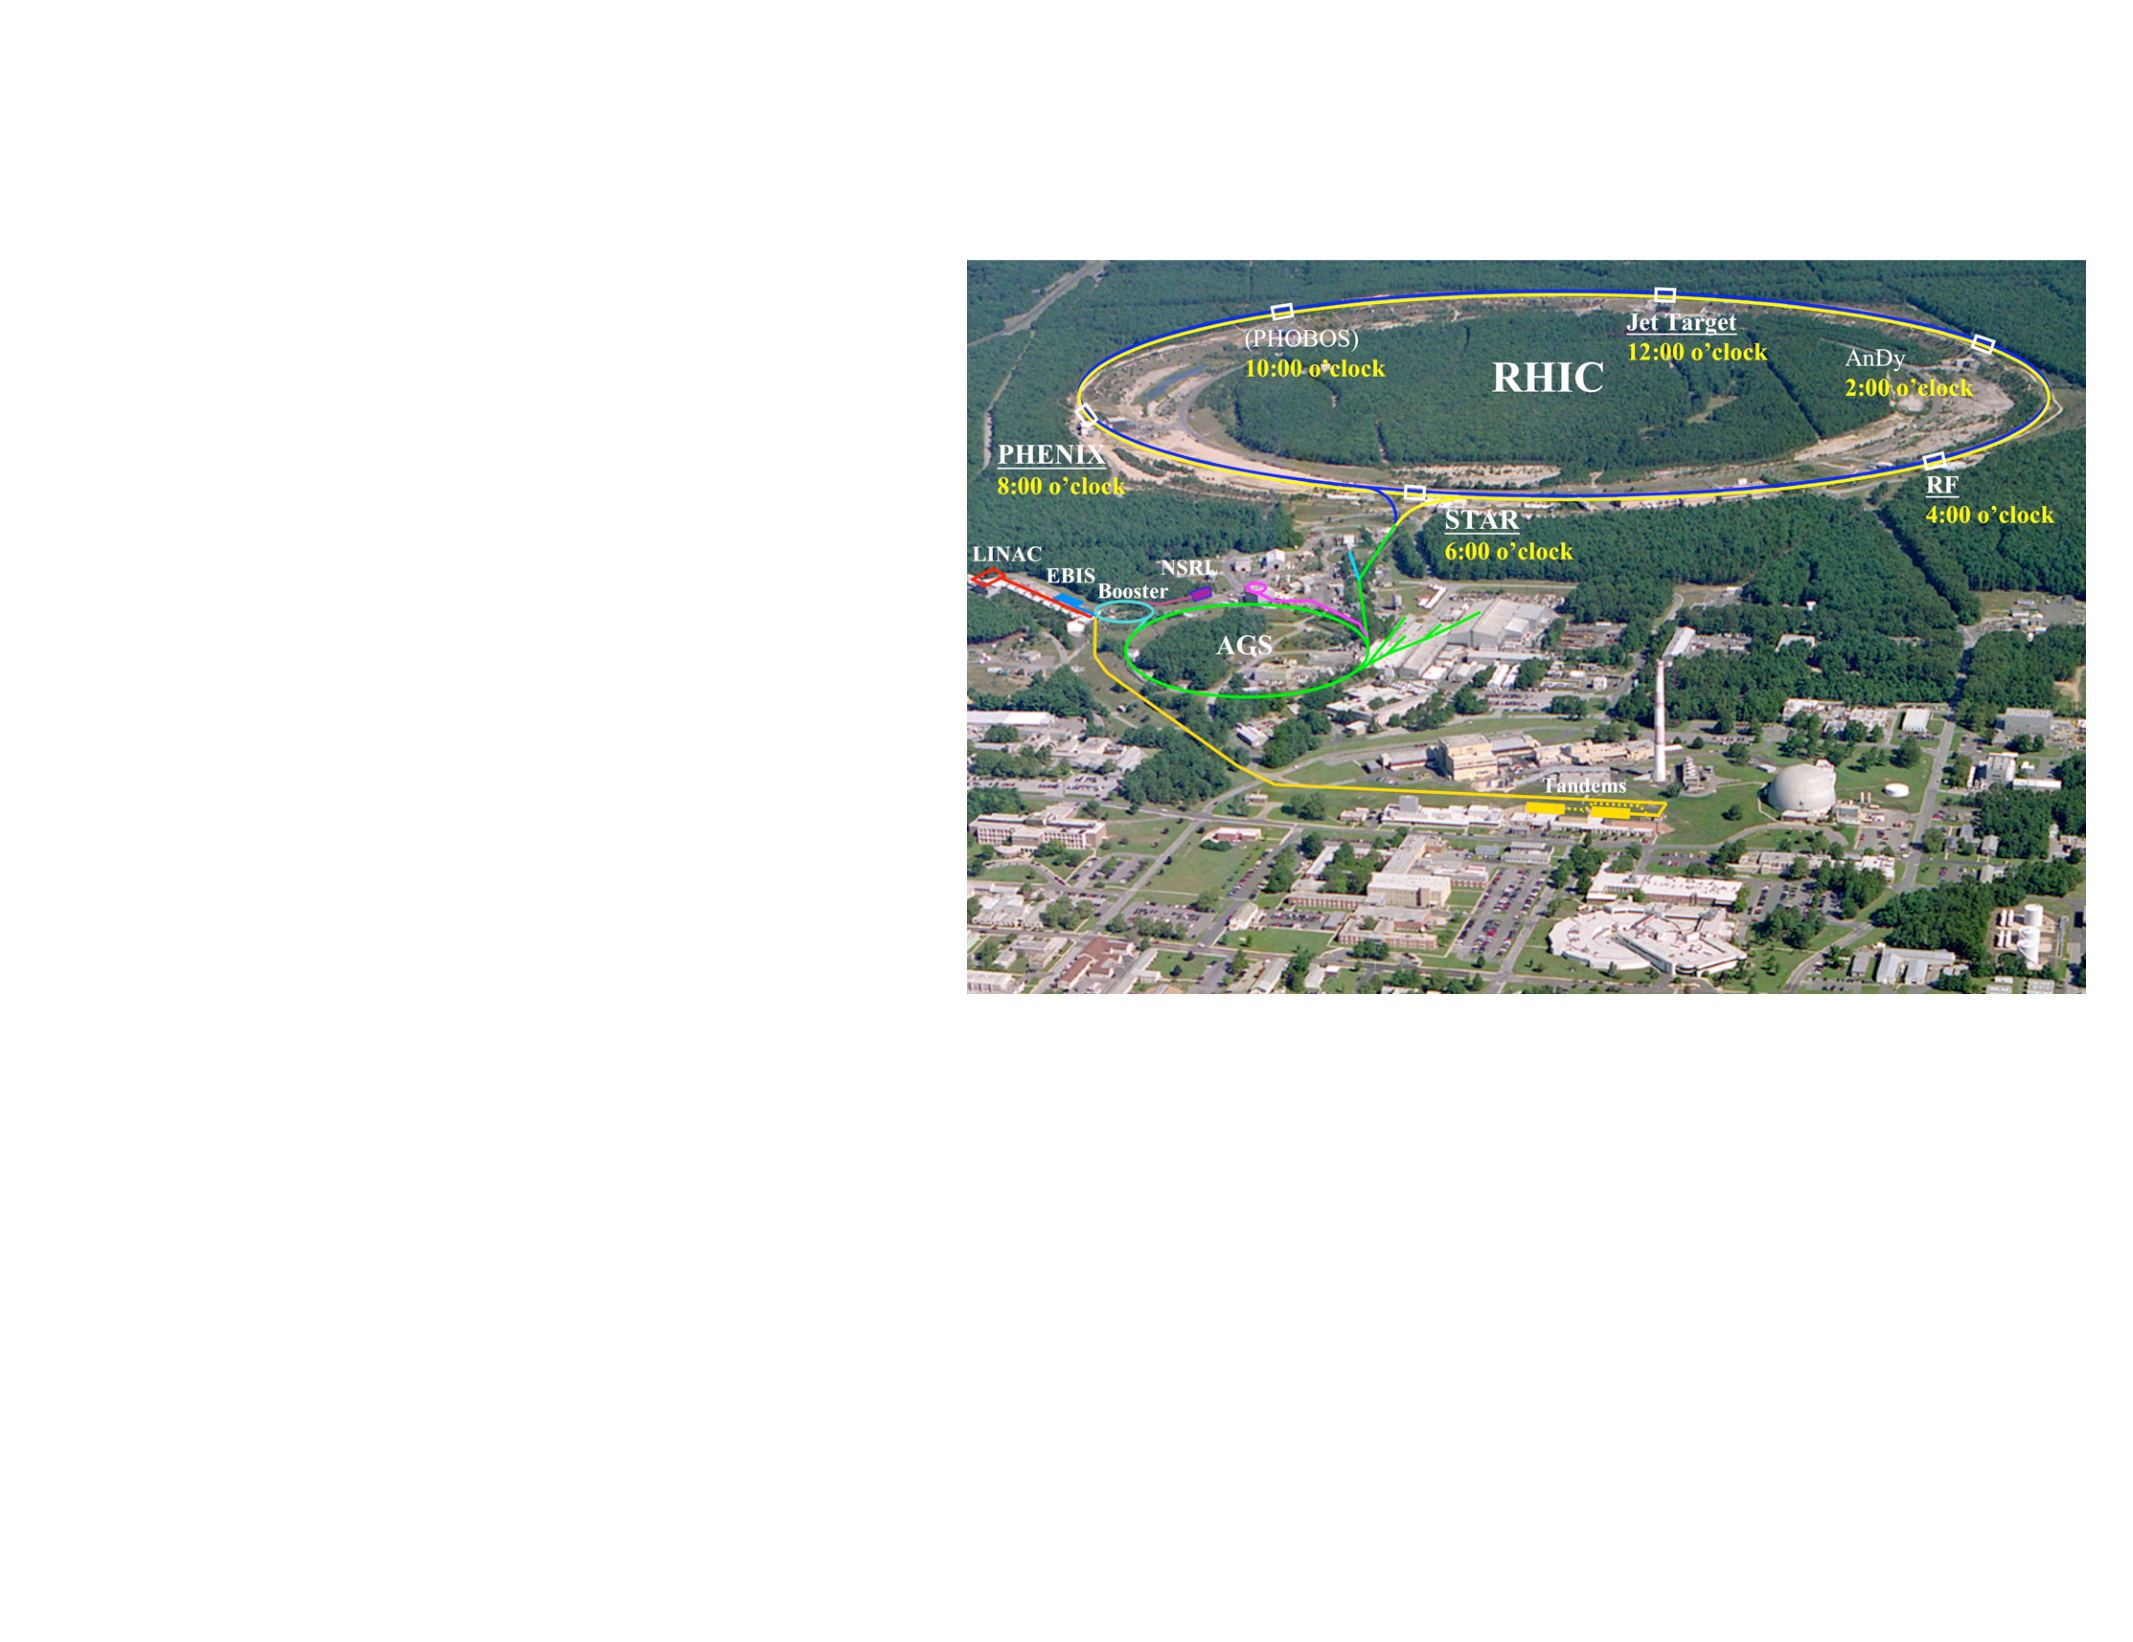
\includegraphics[scale=0.7]{Plots/Detector/RHIC_Complex.pdf}
\end{center}
\caption[RHIC Facility]{RHIC Complex seen from above. Top of the picture shows the main rings and locations of various experiments. Lower part shows the LINAC and booster rings.}
\label{fig:RHIC}
\end{figure}

For the run in 2011 gold nuclei were generated from an ion source and then initially accelerated in the Tandem Van de Graff line. RHIC had multiple Van de Graff accelerators allowing for collisions between mixed nuclei (for example, Au+Cu or d+Au). From 2012 onwards, the function of the tandems was replaced by the Electron Ion Beam Source (EBIS) which generates particles from deuterons to uranium nuclei. Protons beams on the other hand originate from the 200 MeV LINAC. Both protons and other nuclei move to the booster synchrotron which further accelerates the particles using RF waves. After passing through the booster ring the beams then enter the Alternating Gradient Synchrotron (AGS). The AGS was a long running and highly succesful facility at BNL, three Nobel Prizes resulted from research conducted at AGS. Now AGS serves as a final booster ring before sending the beams to the main RHIC rings. 

The beams then reach RHIC where the last remaining electrons are stripped away leaving only the nuclei. In the storage rings the particles circulate in bunches, typically around 110 bunches per ring, and the beams are brought to their collision energy. Top energy for the heavy ion program in 200 GeV per nucleon, higher energies are used in some p+p collisions and RHIC is also capable of colliding at lower energies as is the case in the beam energy scan program which explores the QCD phase diagram.

\section{STAR Detector}

The Solenoidal Tracker at RHIC (STAR) is a general purpose detector located at the 6 o'clock interaction point at RHIC. STAR consists of a variety of detector subsystems which cover a large acceptance region and allow for a variety of physics programs. This analysis will focus only on data taken with STAR's mid rapidity detectors.

\begin{figure}[htbp]
\begin{center}
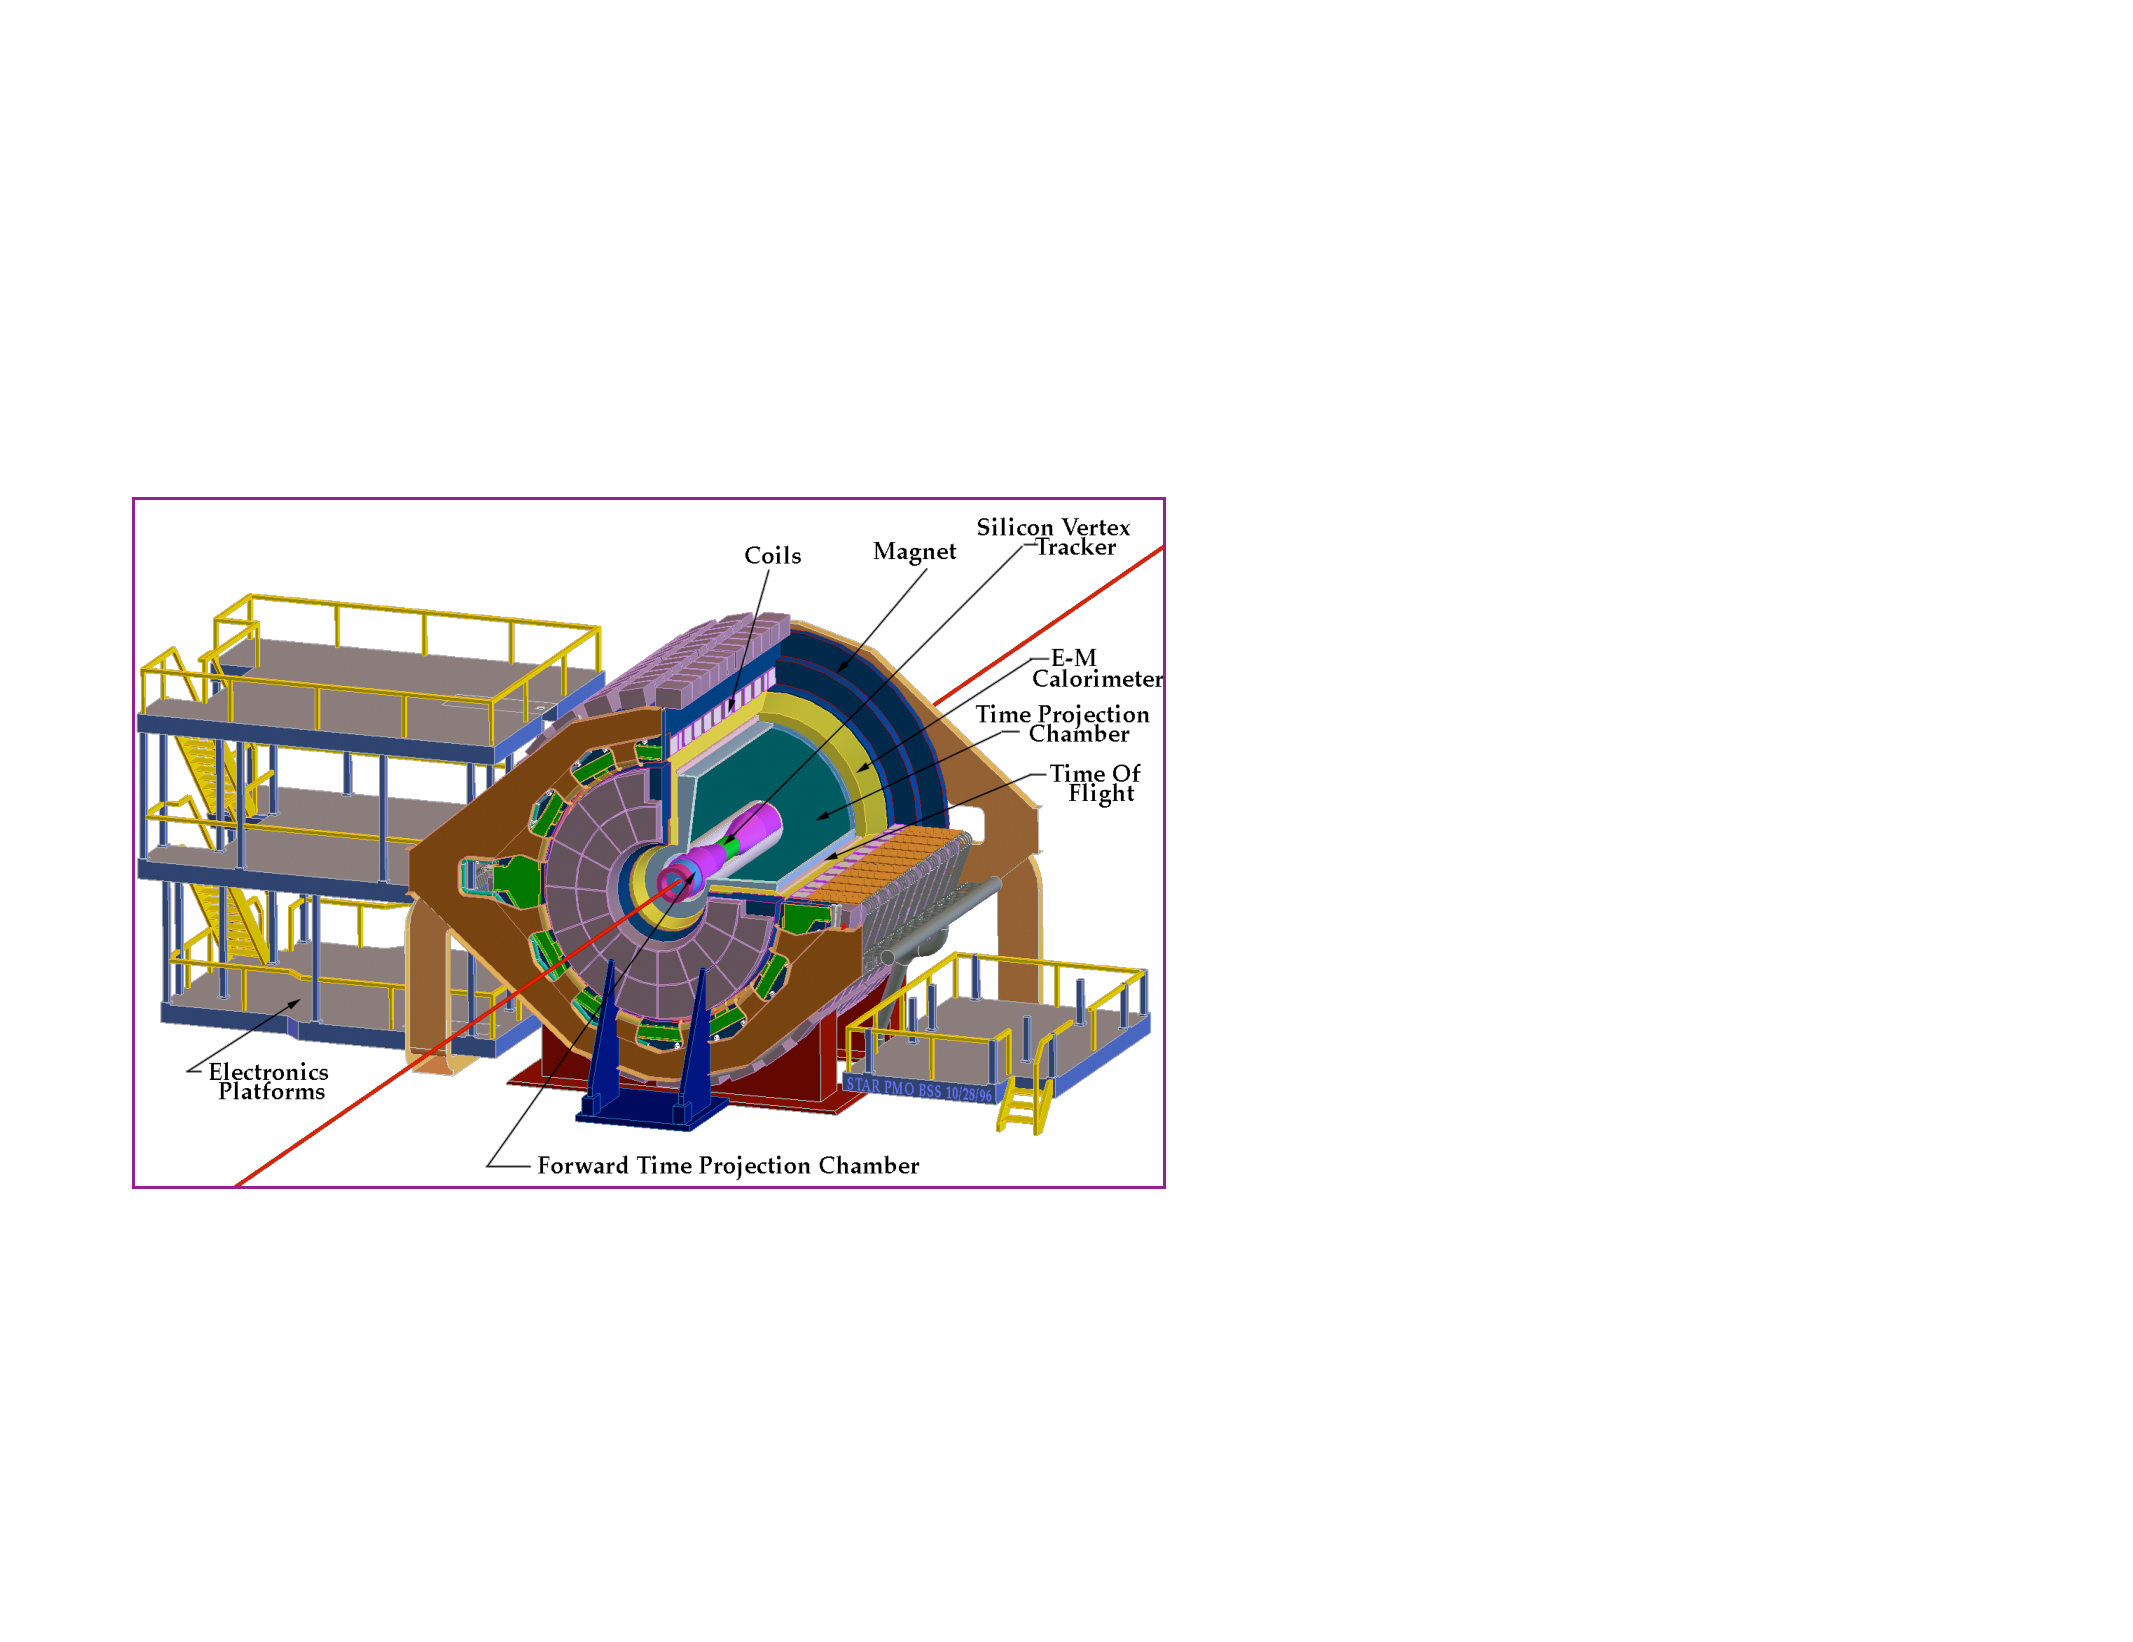
\includegraphics[scale=0.7]{Plots/Detector/STAR_Detector.pdf}
\end{center}
\caption[STAR Detector]{The STAR detector as it was configured around the time of the data taking for this analysis. Of note is that the SVT was removed prior to run 10 and thus only its support structure was in during the runs.}
\label{fig:STAR}
\end{figure}

\section{Time Projection Chamber}

\section{Barrel Electromagnetic Calorimeter}
